\documentclass[letterpaper, 10 pt, conference]{ieeeconf}

\usepackage{graphicx}

\title{\LARGE \bf
A 4-point Algorithm for Relative Pose Estimation of a Calibrated Camera with a Relative Rotation Angle
}

\author{1234}

\begin{document}

\maketitle

\begin{abstract}
We propose an algorithm to estimate relative camera pose using four feature correspondence and one relative rotation angle measurement. The algorithm can be used for relative pose estimation on a vehicle platform mounted with camera and a relative rotation angle sensor, either an odometer or an IMU. This algorithm exploits a fact that relative rotation angle of odometer is invariant under the rigid transform between camera and the rotation sensor. Therefore, extrinsic calibration between camera and sensor is not required. We show that the proposed algorithm improves relative pose estimation compared with the well known 5-point and 1-point algorithm. 
\end{abstract}


\section{Introduction}
Vehicle platform mounted with camera and either a odometer, IMU, or yaw rate sensor has been widely used in research fields of computer vision, robotics and automatic control. For years research has be focused on using these economic sensors to locate the vehicle as well as reconstruct the environment. This research is also referred as Visual SLAM in Robotics. 

The key step of Visual SLAM is to estimate relative camera pose between frame pair. One commonly used method is feature based estimation. A subset of image feature correspondences are selected to estimate the Fundamental Matrix or Essential Matrix between two frames. Relative rotation and translation can then be extracted from the estimation result. A series of ``n-point'' (n-correspondences) algorithms are proposed for this aim. If the camera has with unknown intrinsics, the Fundamental Matrix can be estimated by 8-point [x] or 7-point [x] algorithm. If the camera has calibrated intrinsics, then 6-point [x] or 5-point [x] can be used to the Essential Matrix. Based on these algorithms, robust estimation methods like RANSAC or LMedS are used to generate best estimation from a set of points with both inliers and outliers. The result of ``n-point'' algorithm is significantly affected by the feature correspondences detected from images. It is well admitted that the algorithm using fewer points has lower estimation error. For calibrated camera, 5-point is the minimal case to solve the 5 DoF relative pose. In [x, x], 5-point algorithm shows the best estimation performance compared with 6, 7, 8-point algorithms. For Visual SLAM or Structure from Motion problem, 5-point algorithm is also the most commonly used algorithm if the camera is calibrated. 

However, stable estimation is still not always guaranteed for 5-point algorithm. On a vehicle with camera mounted in its front, relative pose estimation is especially a difficult case for 5-point algorithm. The difficulties include the following: 1) 5-point algorithm less stable in forward motion compared with sideway motion. 2) Features seen by a front camera are mainly far away from the vehicle, which also make the estimation unreliable. Readers can find some discussion about the performance of 5-point algorithm in [x, x]. To improve the estimation quality, research has been drawn on exploiting extra information from other sensors or from specific motion model. For example, [x] obtains two rotation angle from IMU and uses 3 point pairs to estimate the relative pose of a MAV. This method requires that the extrinsic calibration between camera and IMU is known. In [x], a very neat 1-point algorithm was proposed. The algorithm assumes that vehicle platform motion follows the General Ackermann steering model. The 1-point algorithm can work fast and stable for vehicle platform but requires that camera is well align on the rear axis of the vehicle. 

If the vehicle platform has an odometer and its extrinsic parameter is available, it is well known that camera relative pose can be directly obtained from odometer pose $H_o$ as $H^{-1} H_o H$, where $H$ is the transform between camera and odometer. However, in practice estimating $H$ is not easy. This problem is known as Hand-eye (or Head-eye) calibration [x]. Moreover, the success of these hand-eye calibration algorithms also requires accurate visual odometry estimation. This visual odometry estimation also requires pure features algorithm like 5, 6, 7, 8-point algorithms. 

Similarly to [x, x], in this paper we propose a method to improve the relative pose estimation using extra information from odometer. In our algorithm, camera can be mounted anywhere on the platform and no extrinsic calibration is required. The algorithm uses 1 rotation angle from any relative rotation sensor including odometer, IMU, and 4 point pairs from camera. Since odometer reading can be much more stable and accurate, the proposed can largely improve relative estimation compared with existing methods. 

The rest of the paper is organised as follows. Sec.\ref{Preliminaries} establishes notations and formulas used in the proposed methods. Sec.\ref{Algorithm} presents the form of 4-point relative pose problem and the algorithm to solve it. The performance of the algorithm is studied in Sec.\ref{}, where it is compared with the well known 5-point algorithm on both simulated cases to explore how much the algorithm improves 5-point algorithm. Meanwhile, the algorithm is compared with 5-point and 1-point algorithm on a real dataset obtained from our vehicle platform mounted with camera and odometer. 

\section{Preliminaries}
\label{Preliminaries}

Image points from the first and second frame are denoted by homogeneous vectors $p_1 = (x_1, y_1, 1)^\top$ and $p_2 = (x_2, y_2, 1)^\top$, resp. Intrinsic matrix of the camera is denoted as $K$. Since the proposed algorithm requires $K$ to be known, we hereby assume that $p_1$ and $p_2$ are always premultiplied by $K^{-1}$. 

Denote $R$ and $t$ as the relative rotation and translation between the first and second frame. The Essential Matrix corresponding to $R$ and $t$ can be denoted as 
\begin{equation}
\label{EssentialDecomposition}
E = [t]_\times R
\end{equation}
where $[t]_\times$ denotes the skew symmetric matrix
\begin{equation}
[t]_\times \equiv \left(
	\begin{array}{clr}
		0 & -t_3 & t_2 \\
		t_3 & 0 & -t_1 \\
		-t_2 & t_1 & 0
	\end{array}
\right)	
\end{equation}

For correspondence $p_1$, $p_2$, it is well know that
\begin{equation}
\label{EpipolarConstraints}
{p_2}^\top E p_1 = 0
\end{equation}

\textbf{Rodrigues' rotation formula} 
Given a 3D unit rotation axis vector $r = (r_x, r_y, r_z)^\top$ and a rotation angle $\theta$, it is easy to find the the corresponding rotation matrix using Rodrigues' rotation formula. 
\begin{equation}
\label{Rodrigues}
R(\theta, r) = \cos \theta I + (1 - \cos \theta) r r^\top + \sin \theta [ r ]_\times
\end{equation}
where $I$ is a $3 \times 3$ identity matrix. 

\textbf{Theorem}
The rotation angle of camera and odometer is always the same. 

This is a very well known fact for rigid motion. Detailed proof can be found in many textbooks on mechanics. This fact means that relative camera rotation is the same value measured by the relative rotation angle sensor. Note that this angle is the only invariant measurement from the sensor to camera. We do not know the rotation axis of a camera without extrinsic calibration, though in the world frame, it has the same direction with the rotation angle of the sensor. 


\section{Algorithm}
\label{Algorithm}

\subsection{Problem Formation}
Substituting Eq.(\ref{Rodrigues}) into Eq.(\ref{EssentialDecomposition}). We can denote the Essential Matrix as 
\begin{equation}
E(\theta, r, t) = [t]_\times \left( \cos \theta I + (1 - \cos \theta) r r^\top + \sin \theta [ r ]_\times \right)
\end{equation}
where $r$ is a 3D unit vector and $t$ can also be assumed to be unit since it is up to scale. Since we assume that we know $\theta$ from odometer reading, this means that the 5DoF camera relative pose now only have 4 DoF. By using 4 image points correspondences, we can solve $r$ and $t$. 

Thus the equation system for solving relative pose can be form as follows. 
\begin{eqnarray}
\label{ProblemEquation1}
{p_2^i}^\top E(\theta, r, t) p_1^i & = 0,& i = 1, 2, 3, 4 \\
\label{ProblemEquation2}
|| r ||^2 & = 1 & \\
\label{ProblemEquation3}
|| t ||^2 & = 1 &
\end{eqnarray}
where $r = (r_x, r_y, r_z)^\top$ and $t = (t_x, t_y, t_z)^\top$ are six unknowns. 

\subsection{Solution}
\label{Solution}
Equation system (\ref{ProblemEquation1}) includes 4 polynomials with the highest monomial in the form of $t_\star r_\star r_\star$, where $\star$ denotes any arrangement of `$x$', `$y$', `$z$'. Eq.(\ref{ProblemEquation2}) and Eq.(\ref{ProblemEquation3}) are two quadratic polynomials. 

The degree and the number of equations for this equation system is very high  compared with other normal minimal solution problem. In our experiment, we attempted to reduce it using Resualtant Method in Maple. However, this attempt failed as it exceeded the PC memory capacity after one hour running. A working way to solve the system is to use Groebner basis. In our experiment, we use the automatic generator of Groebner solver developed by [x]. After possible simplification, the solver still required executing a Gauss-Jordan elimination on a $270 \times 290$ matrix. In this paper, we proposed a method to use Powell's Hybrid method [] to solve the above equation system. 

Expanding Eq.\ref{ProblemEquation1}, we can denote the equations in the following form. 
\begin{equation}
f_1^i(r_x, r_y, r_z) t_x + f_2^i(r_x, r_y, r_z) t_y + f_3^i(r_x, r_y, r_z) t_z = 0
\end{equation}
where $i = 1, 2, 3, 4$. $f_\star^i$ is a polynomial of $r_x$, $r_y$ and $r_z$. We can further stack $f_\star^i$ into a matrix as follows. 
\begin{equation}
F(r_x, r_y, r_z) t \equiv \left( 
	\begin{array}{clr}
	f_1^1 & f_2^1 & f_3^1 \\
	f_1^2 & f_2^2 & f_3^2 \\
	f_1^3 & f_2^3 & f_3^3 \\
	f_1^4 & f_2^4 & f_3^4 \\	
	\end{array}
\right) \left(
	\begin{array}{clr}
	t_x \\ t_y \\t_z
	\end{array}
\right) = 0	
\end{equation}
Since we assume that $||t||^2 = 1$, the rank of $F$ must be $2$. This means that the determinant of all $3 \times 3$ submatrices must be 0. We form this as follows. 
\begin{eqnarray}
\label{SimplifiedEquation1}
\left| 
	\begin{array}{clr}
	f_1^1 & f_2^1 & f_3^1 \\
	f_1^2 & f_2^2 & f_3^2 \\
	f_1^3 & f_2^3 & f_3^3 \\
	\end{array}
\right| = 0 \\ 
\label{SimplifiedEquation2}
\left| 
	\begin{array}{clr}
	f_1^2 & f_2^2 & f_3^2 \\
	f_1^3 & f_2^3 & f_3^3 \\
	f_1^4 & f_2^4 & f_3^4 \\	
	\end{array}
\right| = 0 
\end{eqnarray}

Combining Eq.(\ref{SimplifiedEquation1}), Eq.(\ref{SimplifiedEquation2}) and Eq.(\ref{ProblemEquation2}), we have a new equation system on $r_x$, $r_y$, $r_z$. Eq.(\ref{SimplifiedEquation1}) and Eq.(\ref{SimplifiedEquation2}) are of 5 degree. Notice that Eq.(\ref{ProblemEquation3}) implies that $(r_x, r_y, r_z)^\top$ is on a unit sphere. We can parametrize it as 2D point and then use gradient descend method like Powell's Hybrid method to find a root from an initial guess. In our experiment, we used $100$ initial guesses drawn by uniform sampling on a unit sphere. This setting could always reaches a proper solution and fails very rarely. After $r_x$, $r_y$, $r_z$ are solved, $F$ is then obtained and $t$ can be solved as the nullvector of $F$. 

Note that for multiple roots $r$ exist for the equation system. For each possible solution $(r, t)$, $(r, -t)$ is also a possible solution. By checking reprojection error e.g. Sampon's error, extra solutions can be rejected till only two solutions $(r, t)$ and $(r, -t)$ remain. The extra solution can then be rejected by checking if the reconstructed 3D points have positive depth. This is also called cheirity check in [x]. 

For a set of correspondences detected from an image pair, methods like RANSAC or LMedS can be used to find the optimal estimation and remove outliers. 

\section{Experiments}
\subsection{Implementation details and timing issues}
As mentioned in Sec.\ref{Solution}, we implemented the 4-point algorithm using Powell's Hybrid method from General Scientific Library (GSL). For each initial guess, the method reached a root or failed within 20 iterations. For the minimal case with four points, this implementation takes XXs on average. In our experiment on a Core i7 desktop, this is enough to process XX image frames per second. 

The computational complexity can be further optimized. The calculation of coefficients in Eq.(\ref{SimplifiedEquation1}) and Eq.(\ref{SimplifiedEquation2}) involves a series extremely large polynomials generated by Maple, which is the computational bottleneck of the current implementation. The computation can be much accelerated by carefully rearrange the polynomial calculation. In addition, the Groebner based solver generated by [x] can also be accelerated with sparse matrix decomposition algorithm. 

The improved implementation of our algorithm will be soon released as open source. 

\subsection{Performance under noise}
We use simulation data in this section to test the performance of the algorithm. For related algorithms including 8-point, 7-point, 6-point and 5-point algorithms, it is well admitted that 5-point algorithm outperforms the others for calibrated camera. Therefore, in this section we only compare our algorithm with 5-point algorithm. Detailed comparison between 8, 7, 6, 5-point algorithms can be found from [x, x]. 

To make our experiment comparable with previous research, we kept our simulation setting close to the challenging condition in [x]. The setting is summarized in Table \ref{SettingTable} and Figure \ref{SettingFigure}. According to [x], relative pose estimation algorithm may have different performance under forward motion and backward motion. Thus we, like in [x, x], tested 4-point and 5-point algorithms under the two motions. Translations for forward and sideway motion are $(1, 0, 0)^\top$ and $(0, 0, 1)^\top$, resp, with $5\%$ noise added. Rotations for the two motions are both $I_{3 \times 3}$ with $5\%$ noise added. Relative pose estimation error is measured by the included angle between groundtruth translation and estimated translation. This is based on the fact that translation estimation is much more sensitive than rotation estimation. Some discussion about this can be found from [x]. Image features noise is generated zero mean Gaussian with increasing standard deviation. For the minimal case test, four and five points are generated for 4-point and 5-point algorithms, resp. For the RANSAC case test, we used 50 point to run a RANSAC scheme to generate the best estimation. $1000$ tests are executed for each noise level in the minimal case test. $100$ tests are executed for each noise level in the RANSAC test. Figure \ref{} shows the plot of estimation error against increasing feature noise standard deviation.  In Figure \ref{}a and \ref{}b, we plotted the lower quantile of error at each noise level for tests of minimal case. In Figure \ref{}c and \ref{}d, we plotted the mean error at each noise level for the RANSAC tests. Note we kept the error estimator consistent with those in [x]. From the plots, we can clearly see the improvement of 4-point algorithm compared with 5-point. 

\begin{table}
\caption{Experiment setting for simulation data. }
\begin{center}
\begin{tabular}{|l|l|}
	\hline	
	Minimal Distance & 10 \\
	\hline
	Depth & 5 \\
	\hline
	Baseline & 1 \\
	\hline
	Image Size & $350 \times 350$ \\ 
	\hline	
	Field of View & 60 deg \\
	\hline	
	Error Measurement & Translation deviation angle \\ 
	\hline	
	Error Estimator & Lower quantile (minimal case) \\
	& Mean (RANSAC case) \\
	\hline
	Tests per Noise Level & 1000 (minimal case) \\
	& 100 (RANSAC case) \\
	\hline	
\end{tabular} 
\end{center}
\label{SettingTable}
\end{table}

\begin{figure}
\begin{center}
	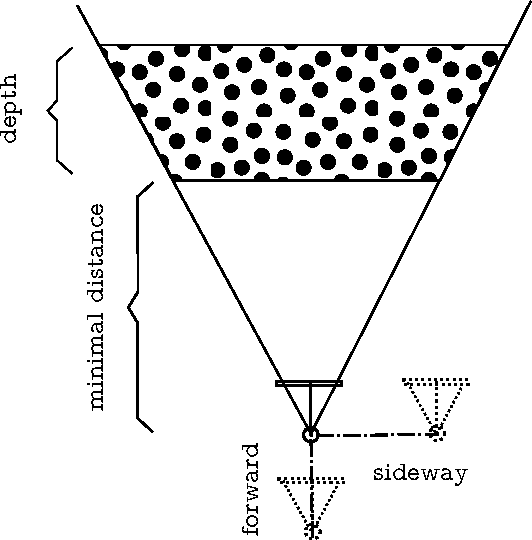
\includegraphics[width=2.5in]{setting.pdf} 
\end{center}
\caption{Experiment setting for simulation data. Two dashed cameras show how camera is moved under forward and sideway motion. }
\label{SettingFigure}
\end{figure}

In addition to the above tests, we provide a test here to show how the four-point algorithm is influenced by the noise from relative rotation angle sensor. Generally it is not straightforward to model the noise of relative rotation angle sensor. Since the rotation angle is usually obtained by integration of the angular velocity, we assume here that a relative rotation angle $\theta$ is measured as $(1 + e) \theta$ by sensor, where $e$ follows a zero mean Gaussian distribution. This test, we selected the standard deviation of $e$ as 0, 0.02, 0.04, 0.06 and 0.08 and generated 5 plots of translation error and noise level. In this tests, we use the same setting with the above tests, except that translation direction is arbitrary and rotation angle is within $-45 \sim 45$ deg. The plot is shown in Fig.\ref{}. We can find that with error rate $e$ smaller than 0.06, four-point algorithm can give a better result than five-point algorithm. In practice, the error rate of rotation sensor is much smaller than that, which guarantees four-point to have a solid performance. 

\end{document}